\documentclass[a4paper]{article}

\usepackage{graphicx}
\usepackage{amsmath}
\usepackage{enumitem}
\setlist[description]{style=unboxed}

\usepackage{tikz}
\usepackage{pgfplots}
\usepackage{circuitikz}

\usetikzlibrary{calc,positioning,shapes,decorations.pathreplacing}

\tikzset{
	short/.style={draw,rectangle,text height=3pt,text depth=13pt,
		text width=7pt,align=center,fill=gray!30},
	long/.style={short,text width=1.5cm},
	verylong/.style={short,text width=4.5cm}
}

\begin{document}
\section*{Task 1}
An underwater habitat controls a remotely-operated submarine by sending the coordinates that the submarine has to traverse in sequence. The 3-dimensional coordinates are organized into triplets, as \textsf{xxx.xxx,yyy.yyy,zzz.zzz;} . Each digit and separating characters ("\textsf{,}" and "\textsf{;}") are encoded as an 8-bit ASCII character. Triplets are concatenated and sent sequentially. This datastream is the input to the modulating system of the transmitter.

The transmitter first organizes the input stream into packets. Each packet consists of a preamble, header, data, CRC-16 hash, and a postamble. The frame structure is illustrated in Figure \ref{fig:packet}.

\begin{figure}[h!]
\centering
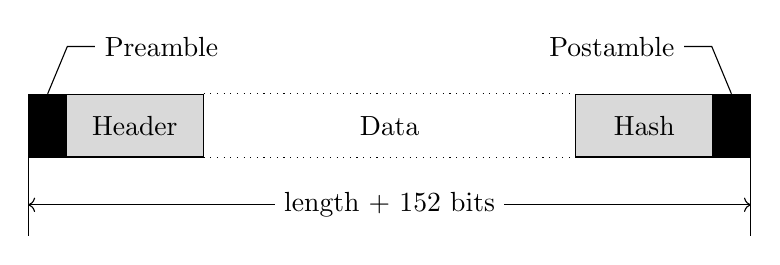
\begin{tikzpicture}[node distance=-\pgflinewidth]

\node[short,fill=black] (preamb) {};
\node[long,right=of preamb,label=center:Header](header){};
\node[verylong,draw=none,fill=none,right=of header,label=center:Data] (data) {};
\node[long,right=of data,label=center:Hash] (hash) {};
\node[short,fill=black,right=of hash] (postamb) {};

\node[above right=0.5cm of preamb] (ppre) {Preamble};
\node[above left=0.5cm of postamb] (ppos) {Postamble};

\draw (ppre.west) -- +(-10pt,0pt) -- (preamb.north);
\draw (ppos.east) -- +(10pt,0pt) -- (postamb.north);
\draw[dotted] (header.north east) -- (hash.north west);
\draw[dotted] (header.south east) -- (hash.south west);
\draw[<->] ( $ (preamb.south west) +(0,-0.6cm) $ ) -- node[fill=white] {length + 152 bits} ( $ (postamb.south east) +(0,-0.6cm) $ );
\draw (preamb.south west) -- +(0,-1cm);
\draw (postamb.south east) -- +(0,-1cm);

\end{tikzpicture}
\caption{Packet structure}
\label{fig:packet}
\end{figure}

Preamble is a predefined 64-bit sequence \textsf{0xa5a5a5a5a5a5a5a5}. Postamble is a bitwise-inverse of the preamble. Header is an 8-bit word containing byte-length of the data section in the packet. The shortest size of the data section is 64 bits, while the largest is 248 bits. The data section is always byte-aligned; i.e. its length is always a multiple of 8 bits.

All the words are stored in packets in big endian notation. The packets are forwarded further in the transmitter chain sequentially, without a guard interval.

The binary sequence of the generated packets is brought to a QPSK modulator. Its constellation is represented by Figure \ref{fig:qpsk}.

\begin{figure}[h!]
\centering
\begin{tikzpicture}
\begin{axis}[
	xmin=-1.5,xmax=1.5,
	ymin=-1.5,ymax=1.5,
	axis lines=center,
	xlabel=$\Re e$,
	ylabel=$\Im m$,
	xtick={-1,...,1},
	ytick={-1,...,1},
]
\addplot+ [nodes near coords, only marks, point meta=explicit symbolic]
table[meta=label]{
	x	y	label
	1	1	00
	-1	1	01
	-1	-1	11
	1	-1	10
};
\end{axis}
\end{tikzpicture}
\caption{QPSK modulator constellation}
\label{fig:qpsk}
\end{figure}

The QPSK-modulated symbols are transposed to carrier frequency $f_c = 36 \,\textrm{kHz}$ and transmitted by a hydrophone. Transmitter data-rate is 9.6 kbit/s. At the receiving end, the receiver aboard a submarine is depicted by a block diagram in Figure \ref{fig:task1}.

\begin{figure}[h!]
\centering
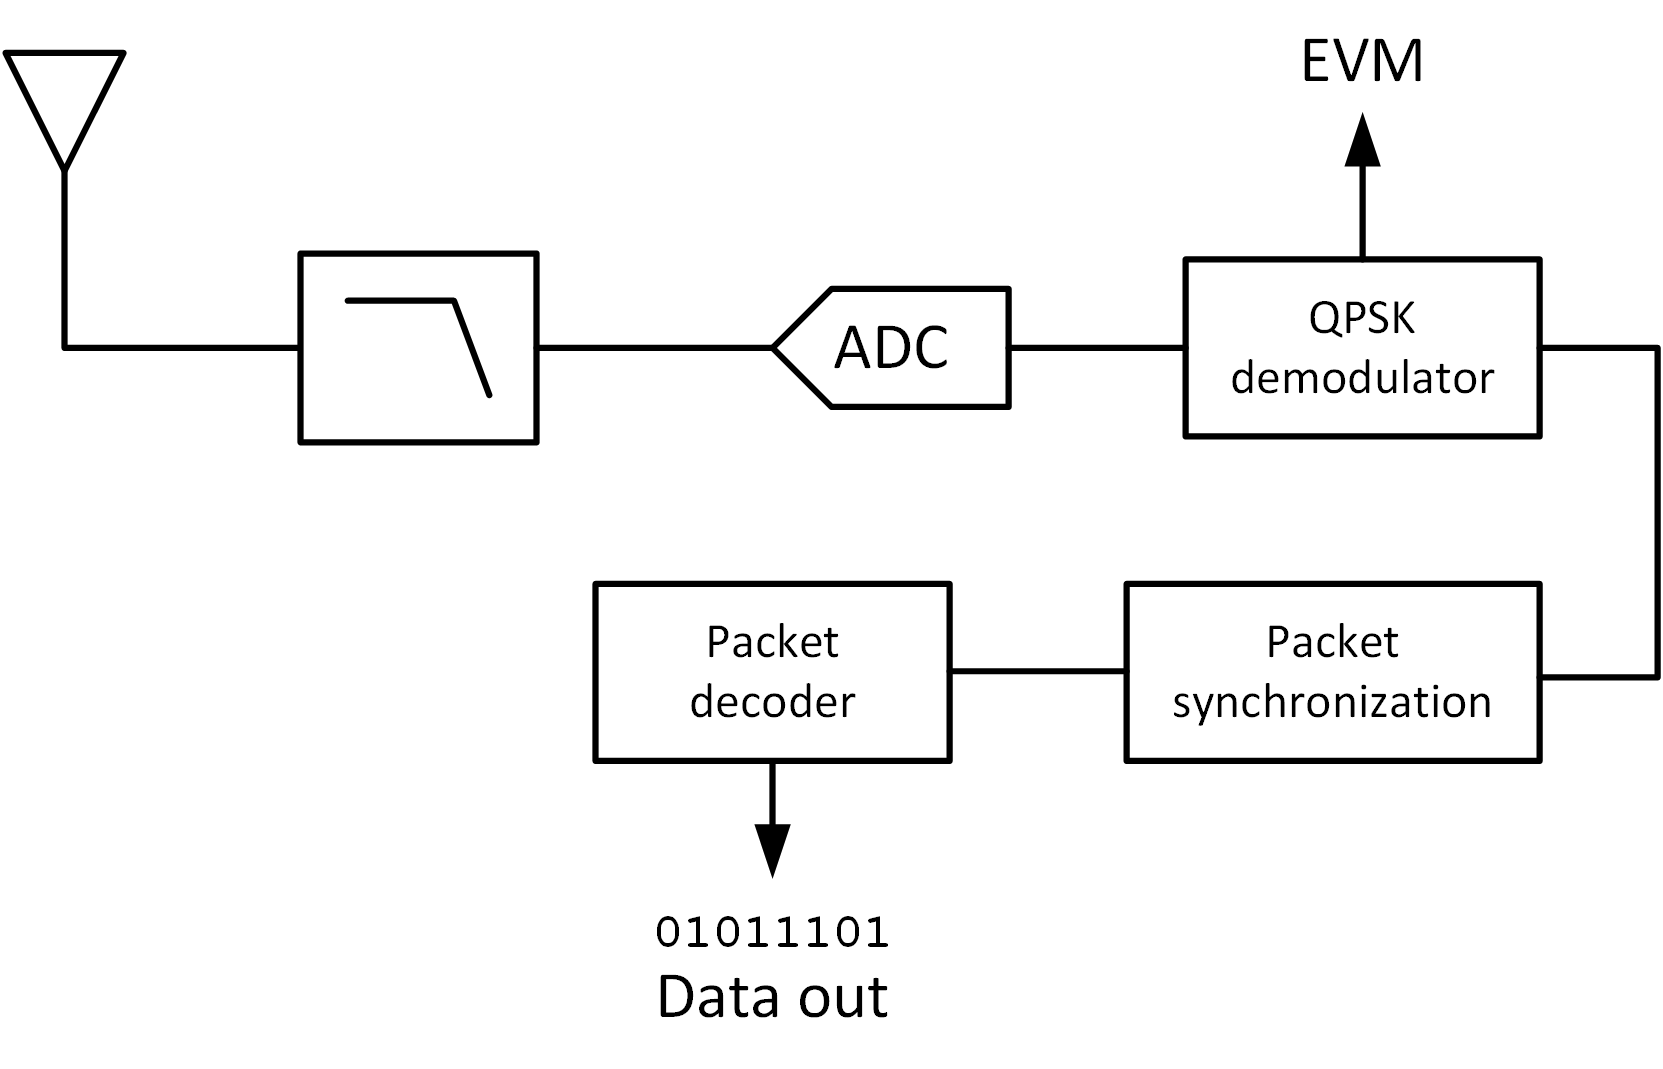
\includegraphics[width=0.9\textwidth]{Task1.png}
\caption{Receiver diagram in Task 1}
\label{fig:task1}
\end{figure}

The ADC of the receiving hydrophone operates at a sampling frequency of 192 kSps. An ideal low-pass filter has a cut-off frequency of 96 kHz.

You are required to implement the digital processing system of the receiver, to demodulate and decode information from the received ultrasonic signal.

\subsection*{Input data}
The \textsf{single\_carrier.raw} file is given. It contains the digitized signal from the ADC, recorded in 16-bit 2's complement format.

\subsection*{Implementation}
Your solution is a C or C++ code implementing the receiver's digital processing chain. You are required to submit at least two files:
\begin{description}
	\item[radio.c / cpp] Implements all the routines described further in the text.
	\item[main.c / cpp] Loads the input data, calls the routines from \textsf{radio.c / cpp}, and outputs decoded data to stdout in the original format.
\end{description}
Should your solution use more source files, you must provide a \textsf{Makefile} that compiles the rest of the source files.

Your radio.c / cpp file must implement the following set of functions:
\begin{description}
	\item[complex *frequency\_shift(double *input, double fc, double fs, int N)]
	\,\\ Transposes the signal provided in input from centre frequency \textsf{fc} to baseband. \textsf{N} is the length of the data stream, expressed as a number of double words. \textsf{fs} is the sampling frequency.
	\item[double qpsk\_demodulator(complex symbol, double constellation\_offset, char *decoded\_symbol)]
	\,\\ Decodes a QPSK symbol \textsf{symbol} to a word, stored in an 8-bit format to \textsf{decoded\_symbol}. The function outputs the EVM of the symbol.
	\item[char *bitstream\_to\_bytestream(char *bitstream, int length)]
	\,\\ Converts \textsf{length} 8-bits words, as output by the previous function, into a bytestream. A pointer to the beginning of the bytestream is returned.
	\item[void frame\_sync(char **bytestream, int length)]
	\,\\ Moves the pointer \textsf{*bytestream} to the beginning of the first detected frame. \textsf{length} is the length of the bytestream.
	\item[int frame\_decoder(char *bytestream, char **data)]
	\,\\ Decodes the data from a single frame that starts at the pointer \textsf{*bytestream}. Data is stored to \textsf{*data}. The return value is the length of processed data (frame length).
\end{description}

You are provided with some helper files:
\begin{description}
	\item[radio.h]
	\item[api.h]
	\,\\ An API containing some types, functions and constants you may find useful.
	\item[api.c]
	\,\\ The compiled API described in \textsf{api.h}.
\end{description}


\section*{Task 2}

Along the submarine's trajectory information, the habitat and the submarine exchange location data on debris scattered around the sea. This data is transmitted in a separate data stream from the trajectory coordinates, but has the same triplet format, as the data from Task 1. The data is packaged in the same manner as in Task 1. The resulting bitstream is then spread into 4 QPSK subcarriers, as depicted in Figure \ref{fig:spread}.
\begin{figure}[h!]
	\centering
	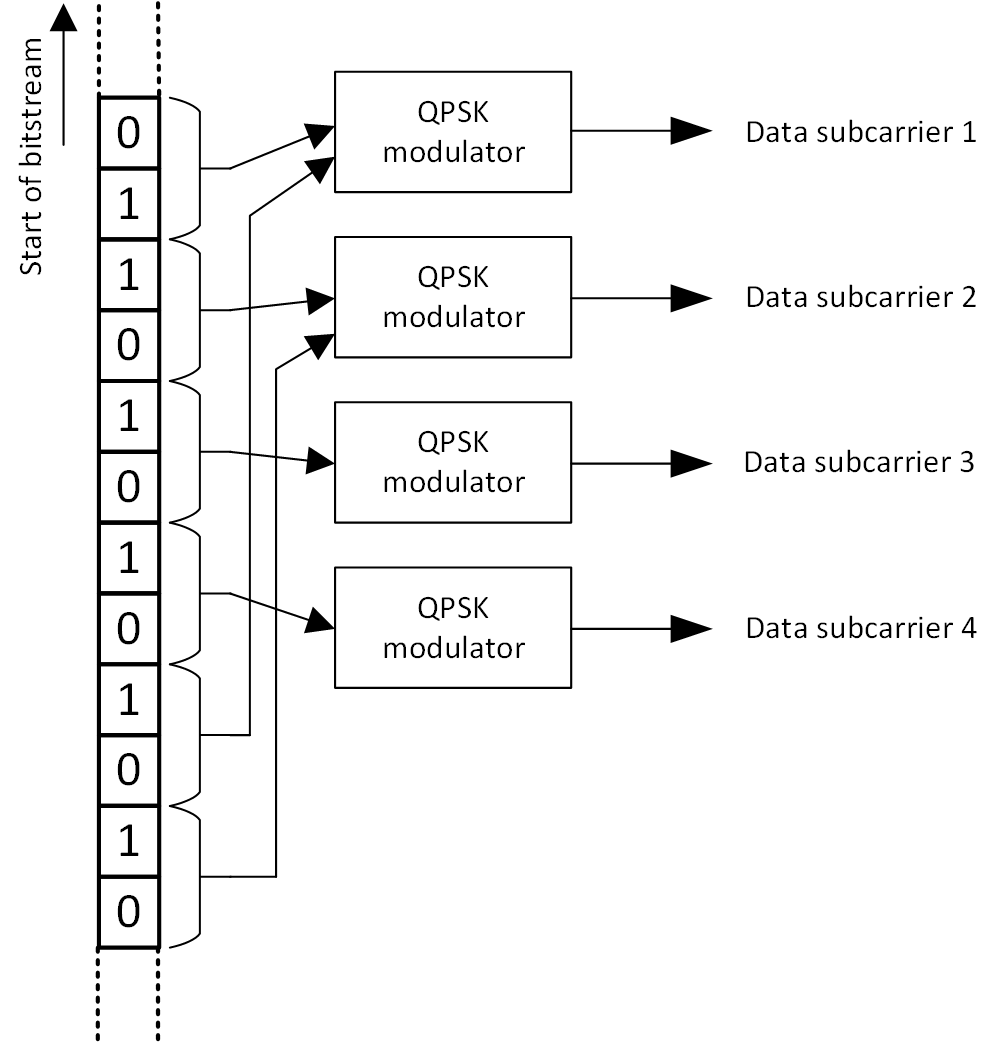
\includegraphics[width=0.7\textwidth]{spread.png}
	\caption{Bitstream spreading mechanism}
	\label{fig:spread}
\end{figure}

The obtained QPSK carriers are multiplexed into OFDM that consists of a total of 10 subcarriers. These are organized as depicted by DFT spectrum in Figure \ref{fig:dft}.
\begin{figure}[h!]
	\centering
	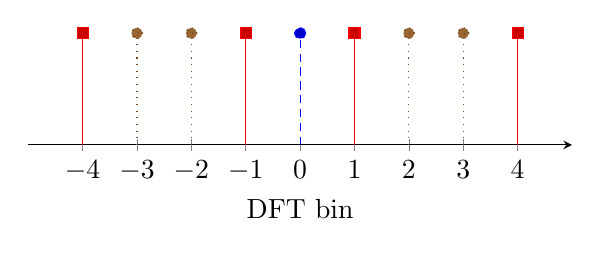
\begin{tikzpicture}
	\begin{axis}[
		width=0.7\textwidth,
		height=3cm,
		axis x line=bottom,
		axis y line=none,
		xlabel=DFT bin,
		ymin=0,ymax=1,
		xmin=-5,xmax=5,
		xtick={-4,...,4}
	]
	% Osnovni podatak
	\addplot+ [ycomb, style={densely dashed}] plot coordinates {
		(0,1)
	};
	% Piloti
	\addplot+ [ycomb, style={solid}] plot coordinates {
		(-4,1) (-1,1) (1,1) (4,1)
	};
	% Ostali nosioci
	\addplot+ [ycomb, style={dotted}] plot coordinates {
		(-3,1) (-2,1)
		(2,1) (3,1)
	};
	\end{axis}
	\end{tikzpicture}
	\caption{OFDM carrier DFT spectrum}
	\label{fig:dft}
\end{figure}

Subcarrier spacing is $\varDelta f = 1500 \,\textrm{Hz}$. The graph is centred to frequency $f_c = 36 \,\textrm{kHz}$, corresponding to the central frequency of the OFDM carrier. The subcarrier at bin 0, depicted by a dashed line, containes trajectory coordinate stream from Task 1. Subcarriers depicted by dotted lines contain the added data stream. Subcarriers depicted by a solid line are pilots. OFDM symbols have no cyclic prefix.

The receiver code from Task 1 has to be modified to work with an OFDM carrier, and decode the additional data stream. Block diagram of the receiver is presented in Figure \ref{fig:task2}.

\begin{figure}[h!]
\centering
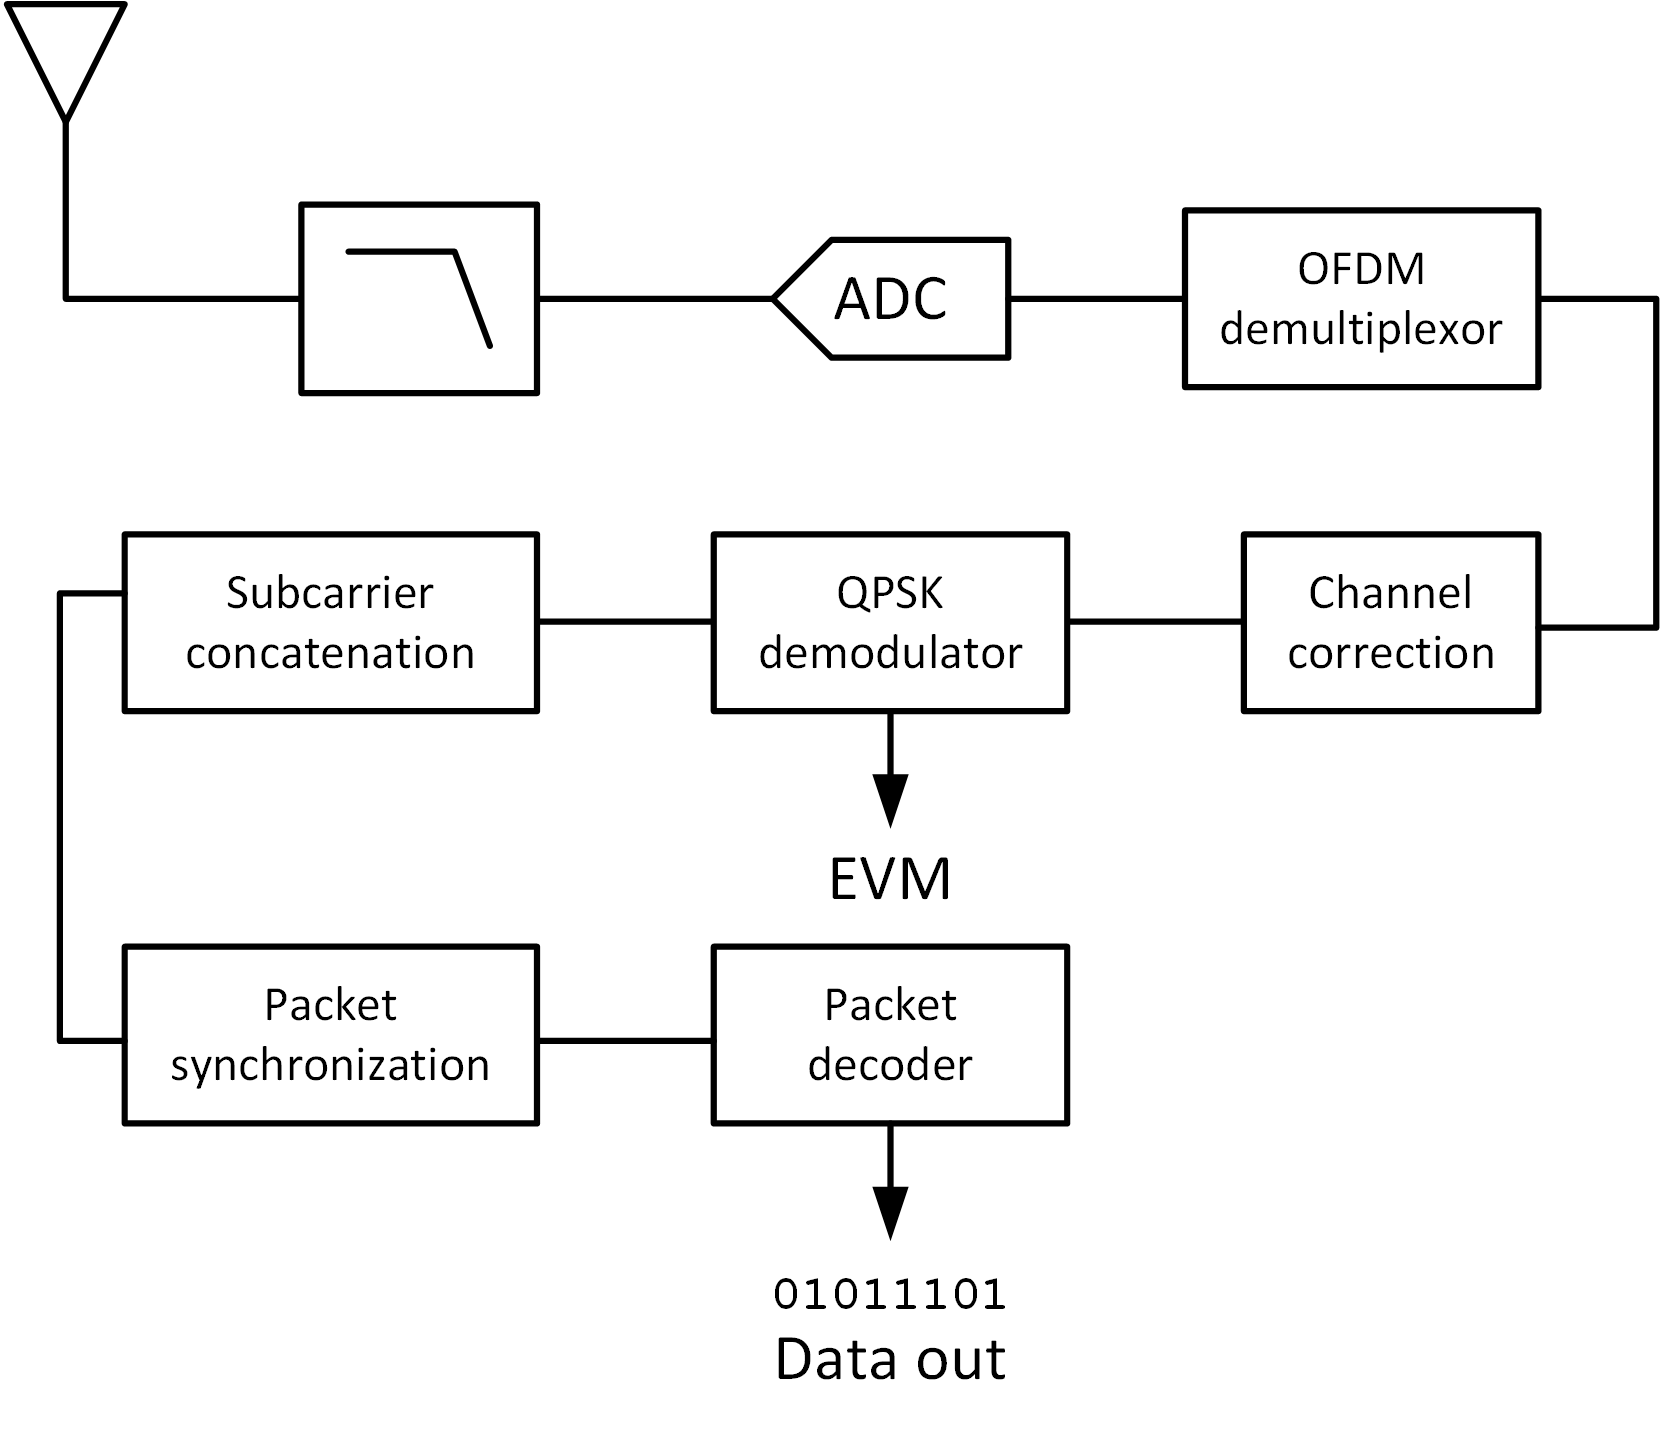
\includegraphics[width=0.9\textwidth]{Task2.png}
\caption{Receiver diagram in Task 2}
\label{fig:task2}
\end{figure}

\subsection*{Input data}
The \textsf{ofdm\_carrier.raw} file is given. It contains the digitized signal from the ADC, recorded in 16-bit 2's complement format.

\subsection*{Implementation}
You should update your \textsf{radio.c / cpp} and \textsf{main.c / cpp} to implement the new features required for Task 2. Your \textsf{radio.c / cpp} file should implement the following additional functions:
\begin{description}
	\item[double *ofdm\_demodulator(complex *input, int *carrier\_idx, int carrier\_no, char **data)]
	\,\\ Demultiplexes the \underline{additional data stream} from the OFDM carrier given in \textsf{input}, and stores it into \textsf{*data}. The input signal is in baseband in the original sample rate. \textsf{carrier\_idx} is a list of DFT bins that contain the additional data stream. \textsf{carrier\_no} is the length of \textsf{carrier\_idx} array.
\end{description}

\section*{Task 3}
An algorithm for calculating the CRC-16 hash of an input stream should be added to solutions for both tasks. CRC-16 verification should first be implemented as a separate function, and then integrated into the receiver chain. The modification is presented in Figure \ref{fig:task3}.

\begin{figure}[h!]
\centering
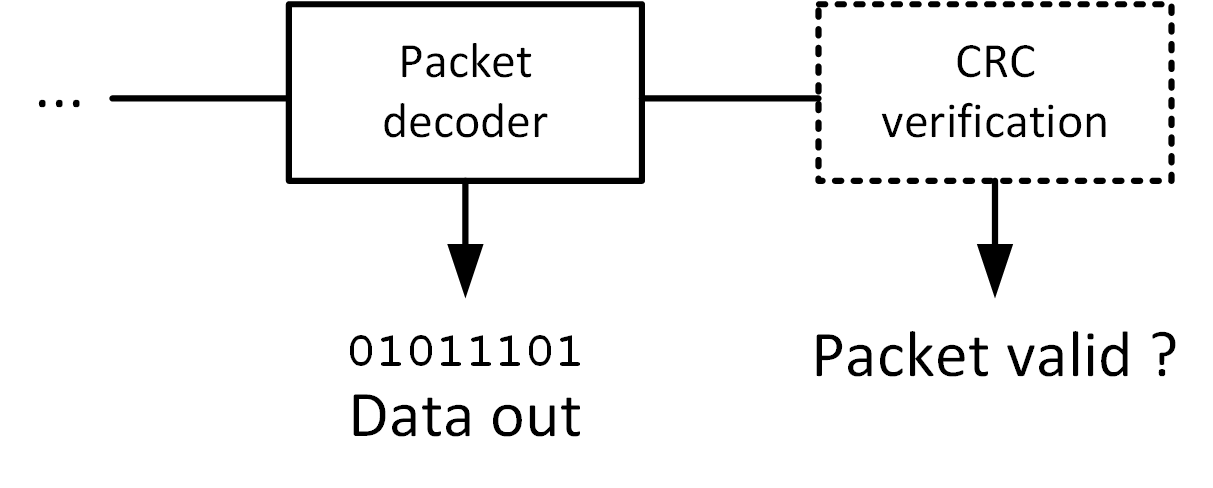
\includegraphics[width=0.7\textwidth]{Task3.png}
\caption{CRC check in receivers}
\label{fig:task3}
\end{figure}

The CRC-16 hash in data frames is calculated using the CRC-CCITT algorithm, with an initial register state \textsf{0xffff}.

\subsection*{Implementation}
Your \textsf{radio.c / cpp} code must implement the following \underline{additional} functions:
\begin{description}
	\item[char crc16\_check(char* bitstream, int length)]
	\,\\ Returns CRC-16 hash of the given \textsf{bitstream}, of length \textsf{length}.
	%\item[int frame\_decoder\_valid(char* bytestream, char** data, bool *valid)]
	%\,\\ Decodes the data from a single frame that starts at the pointer \textsf{*bytestream}. Data is stored to \textsf{*data}. The return value is the length of processed data (frame length).
\end{description}

\section*{Documentation}

Provide documentation that describes your solution for the receiving chain. Back your implementation by describing the mathematical background of your processing chain. Document the datasets you used to evaluate your solution.

The documentation will not be graded, but it can help mentors in understanding your approach and validating the theory behind your solution.

\end{document}
